%==============================================================================
% Sjabloon poster bachproef
%==============================================================================
% Gebaseerd op document class `a0poster' door Gerlinde Kettl en Matthias Weiser
% Aangepast voor gebruik aan HOGENT door Jens Buysse en Bert Van Vreckem

\documentclass[a0,portrait]{hogent-poster}

% Info over de opleiding
\course{Bachelorproef}
\studyprogramme{toegepaste informatica}
\academicyear{2023-2024}
\institution{Hogeschool Gent, Valentin Vaerwyckweg 1, 9000 Gent}

% Info over de bachelorproef
\title{Competitief sportplatform met gamification zodat werknemers in een sedentaire job meer bewegen}
\subtitle{Een proof of concept}
\author{Sarah Eggermont}
\email{sarah.eggermont@student.hogent.be}
\supervisor{Sebastiaan Labijn}
\cosupervisor{Guillaume Vande Maele (we are)}

% Indien ingevuld, wordt deze informatie toegevoegd aan het einde van de
% abstract. Zet in commentaar als je dit niet wilt.
\specialisation{Mobile \& Enterprise developer}
\keywords{Gamification, sportplatform, gezondheid}
% \projectrepo{https://github.com/user/repo}

\begin{document}

\maketitle

\begin{abstract}

Beweging speelt een grote rol in zowel de fysieke als de mentale gezondheid van mensen. Bijna één derde van de wereldbevolking beweegt te weinig en ondervindt hier vroeg of laat de nadelen van. Om die reden bespreekt dit onderzoek of een sportplatform, dat gebruik maakt van gamification, gebruikt kan worden om medewerkers van \href{https://en.joule.be/}{Joule}, \href{https://www.ventures4growth.com/en}{Ventures 4 Growth}, \href{https://www.mace-legal.com/}{mace}, \href{https://planetb.life/en}{PlanetB}, \href{https://www.we-are.be/}{we are} en \href{https://www.delaware.pro/en-be}{delaware}, die een sedentaire job beoefenen, aan te zetten om meer te sporten.

Na een literatuurstudie rond het belang van beweging, gamification en hoe gamification de intrinsieke motivatie om te bewegen kan bevorderen, worden werknemers van eerder genoemde bedrijven geïnterviewd om de succescriteria en de benodigdheden van het nieuwe platform te bepalen. Aan de hand van deze criteria wordt een platform, in de vorm van een responsive website, gecreëerd. In deze proof of concept wordt gamification geïmplementeerd en worden sportgegevens van deelnemende werknemers verzameld en grafisch voorgesteld op het platform. Tegelijkertijd wordt ook de beleving omtrent het gamification-aspect bevraagd. Deze gegevens leiden, samen met de eerder verzamelde data, tot de conclusie van dit onderzoek.

Dit onderzoek suggereert dat een sportplatform met gamification wel degelijk zorgt voor een verbetering in de hoeveelheid beweging van mensen in een sedentaire job. Daarnaast stelt het dat gamificationtechnieken zoals punten en scoreborden, vooral wanneer dit zorgt voor een onderlinge competitie, het meest succesvol zijn. Tenslotte zijn er in dit onderzoek geen gamificationtechnieken opgemerkt die een negatief effect hebben op de hoeveelheid beweging van gebruikers, maar moet wel opgemerkt worden dat, binnen de context van een sportapplicatie, personen het storend vinden om meldingen te ontvangen als deel van de gamification.

\end{abstract}

\begin{multicols}{2} % This is how many columns your poster will be broken into, a portrait poster is generally split into 2 columns

\section{Introductie}

Be quiet! Found them? In Mercia?! The coconut's tropical! But you are dressed as one… Well, what do you want? Knights of Ni, we are but simple travelers who seek the enchanter who lives beyond these woods.

Well, what do you want? It's only a model. Camelot! We found them. We shall say `Ni' again to you, if you do not appease us.

The nose? Shut up! Burn her! I am your king. You don't vote for kings.

You can't expect to wield supreme power just `cause some watery tart threw a sword at you! Well, we did do the nose. I don't want to talk to you no more, you empty-headed animal food trough water! I fart in your general direction! Your mother was a hamster and your father smelt of elderberries! Now leave before I am forced to taunt you a second time!

Why do you think that she is a witch? We want a shrubbery!! I don't want to talk to you no more, you empty-headed animal food trough water! I fart in your general direction! Your mother was a hamster and your father smelt of elderberries! Now leave before I am forced to taunt you a second time!

\section{Experimenten}

A newt? Camelot! Why? No, no, no! Yes, yes. A bit. But she's got a wart.

Shut up! I dunno. Must be a king. Who's that then? Look, my liege! On second thoughts, let's not go there. It is a silly place.

Shut up! Will you shut up?! No, no, no! Yes, yes. A bit. But she's got a wart. He hasn't got shit all over him. It's only a model. It's only a model.

Bring her forward! I don't want to talk to you no more, you empty-headed animal food trough water! I fart in your general direction! Your mother was a hamster and your father smelt of elderberries! Now leave

\section{Sectie met figuur}

De {\LaTeX} figure-omgeving bepaalt zelf waar een afbeelding komt en dat is meestal niet op de plek in de tekst waar de figure-omgeving gedefinieerd wordt. Als je wilt forceren dat afbeeldingen toch in de flow van de tekst blijven, dan kan je dat zoals hieronder:

\begin{center}
  \captionsetup{type=figure}
  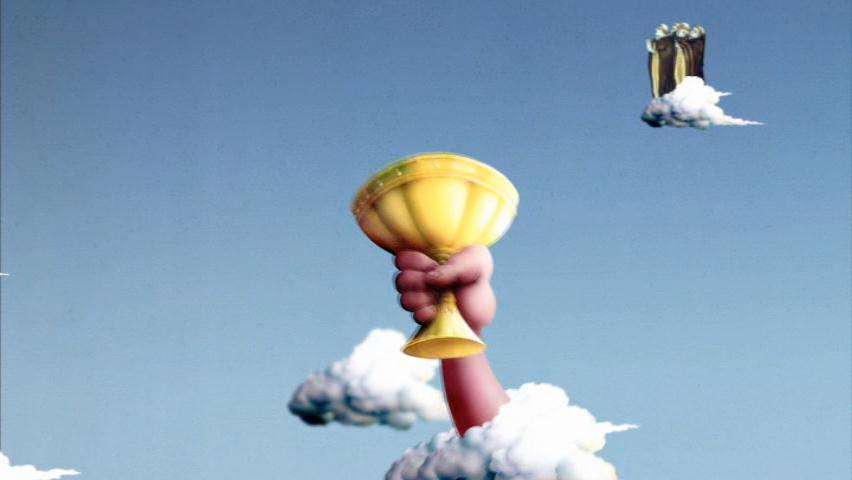
\includegraphics[width=1.0\linewidth]{grail}
  \captionof{figure}{He hasn't got shit all over him. The nose? Where'd you get the coconuts? What do you mean? We shall say `Ni' again to you, if you do not appease us}
\end{center}

Let er wel op dat dit tot problemen met bladschikking kan leiden.

\section{Conclusies}

Don't underestimate the Force. Oh God, my uncle. How am I ever gonna explain this? I suggest you try it again, Luke. This time, let go your conscious self and act on instinct. Don't be too proud of this technological terror you've constructed. The ability to destroy a planet is insignificant next to the power of the Force.

\section{Toekomstig onderzoek}

I care. So, what do you think of her, Han? No! Alderaan is peaceful. We have no weapons. You can't possibly… I have traced the Rebel spies to her. Now she is my only link to finding their secret base.

Kid, I've flown from one side of this galaxy to the other. I've seen a lot of strange stuff, but I've never seen anything to make me believe there's one all-powerful Force controlling everything. There's no mystical energy field that controls my destiny. It's all a lot of simple tricks and nonsense. You are a part of the Rebel Alliance and a traitor! Take her away!

\end{multicols}
\end{document}